%\documentclass[first,firstsupp,handout,compress,notes,navigation]{ETHclass}
%\documentclass[first,firstsupp,handout,lastsupp]{ETHclass}
%\documentclass[first, handout,notes]{ETHclass}
%\documentclass[first,firstsupp,handout,last]{ETHclass}
\documentclass[first,firstsupp,notes, handout, last]{ETHclass}
%\documentclass[first,firstsupp]{ETHclass}

% use sensible encoding
\usepackage[T1]{fontenc}

%% Input encoding 'utf8'. In some cases you might need 'utf8x' for
%% extra symbols. Not all editors, especially on Windows, are UTF-8
%% capable, so you may want to use 'latin1' instead.
\usepackage[utf8x]{inputenc}

\usepackage{pifont}

%% The AMS-LaTeX extensions for mathematical typesetting.  Do not
%% remove.
\usepackage{amsmath,amssymb,amsfonts,mathrsfs}

\usepackage{amsthm}
%% additional package extending mathematical typesetting.
\usepackage{thmtools}
\usepackage{thm-restate}

\usepackage{textpos}

% for graphics
\usepackage{tikz}
\usetikzlibrary{decorations.pathreplacing}
\usetikzlibrary{arrows, decorations.markings}
% for double arrows a la chef
% adapt line thickness and line width, if needed
\tikzstyle{vecArrow} = [thick, decoration={markings,mark=at position
   1 with {\arrow[semithick]{open triangle 60}}},
   double distance=1.4pt, shorten >= 5.5pt,
   preaction = {decorate},
   postaction = {draw,line width=1.4pt, white,shorten >= 4.5pt}]
\tikzstyle{innerWhite} = [semithick, white,line width=1.4pt, shorten >= 4.5pt]
\usetikzlibrary{decorations.shapes}

%% Some more packages that you may want to use.  Have a look at the
%% file, and consult the package docs for each.
%% See the TeXed file for more explanations

%% [OPT] Multi-rowed cells in tabulars
%\usepackage{multirow}

%% [REC] Intelligent cross reference package. This allows for nice
%% combined references that include the reference and a hint to where
%% to look for it.
\usepackage{varioref}

%% [OPT] Easily changeable quotes with \enquote{Text}
%\usepackage[german=swiss]{csquotes}

%% [REC] Format dates and time depending on locale
\usepackage{datetime}

%% [OPT] Provides a \cancel{} command to stroke through mathematics.
%\usepackage{cancel}

%% [NEED] This allows for additional typesetting tools in mathmode.
%% See its excellent documentation.
\usepackage{mathtools}

%% [ADV] Conditional commands
%\usepackage{ifthen}

%% [OPT] Manual large braces or other delimiters.
%\usepackage{bigdelim, bigstrut}

%% [REC] Alternate vector arrows. Use the command \vv{} to get scaled
%% vector arrows.
%\usepackage[h]{esvect}

%% [NEED] Some extensions to tabulars and array environments.
\usepackage{array}

%% [OPT] Postscript support via pstricks graphics package. Very
%% diverse applications.
%\usepackage{pstricks,pst-all}

%% [?] This seems to allow us to define some additional counters.
%\usepackage{etex}

%% [ADV] XY-Pic to typeset some matrix-style graphics
%\usepackage[all]{xy}

%% [OPT] This is needed to generate an index at the end of the
%% document.
%\usepackage{makeidx}

%% [OPT] Fancy package for source code listings.  The template text
%% needs it for some LaTeX snippets; remove/adapt the \lstset when you
%% remove the template content.
\usepackage{listings}
\lstset{language=TeX,basicstyle={\normalfont\ttfamily}}

%% [REC] Fancy character protrusion.  Must be loaded after all fonts.
\usepackage[activate]{pdfcprot}

%% [REC] Nicer tables.  Read the excellent documentation.
\usepackage{booktabs}

%%pseudocode and algorithms
\usepackage{algpseudocode}
\usepackage{algorithm}

%% define comments in single line
\algnewcommand{\LineComment}[1]{\State \(\triangleright\) #1}

%%placing in the right place
\usepackage{float}

\usepackage{caption}

\DeclareCaptionFormat{algor}{
  \hrulefill\par\offinterlineskip\vskip1pt
    \textbf{#1#2}#3\offinterlineskip\hrulefill}
\DeclareCaptionStyle{algori}{singlelinecheck=off,format=algor,labelsep=space}
\captionsetup[algorithm]{style=algori}

\algnewcommand\algorithmicinput{\textbf{Input:}}
\algnewcommand\Input{\item[\algorithmicinput]}

\algnewcommand\algorithmicauxinput{\textbf{Auxiliary input:}}
\algnewcommand\AuxInput{\item[\algorithmicauxinput]}

%indention in algorithms
\newcommand{\pushcode}[1][1]{\hskip\dimexpr#1\algorithmicindent\relax}

% hyphen in math mode
\def\hyph{\text{-}}



%% Theorem-like environments

%% This can be changed according to language. You can comment out the ones you
%% don't need.

\numberwithin{equation}{chapter}

% declare theorem style
\declaretheoremstyle[
spaceabove=6pt, spacebelow=6pt,
headfont=\normalfont\bfseries,
notefont=\mdseries, notebraces={(}{)},
bodyfont=\normalfont\itshape,
postheadspace=1em,
%qed=\qedsymbol
]{thm_sty}

% declare definition style
\declaretheoremstyle[
spaceabove=6pt, spacebelow=6pt,
headfont=\normalfont\bfseries,
notefont=\mdseries, notebraces={(}{)},
bodyfont=\normalfont,
postheadspace=1em,
qed=\ensuremath{\lozenge}
]{def_sty}


%% English variants
\declaretheorem[style=thm_sty, name=Theorem, numberwithin=chapter]{theorem}
\declaretheorem[style=thm_sty, name=Observation, sibling=theorem]{observation}
\declaretheorem[style=thm_sty, name=Lemma, sibling=theorem]{lemma}
\declaretheorem[style=def_sty, name=Definition, sibling=theorem]{definition}
%\declaretheorem[style=def_sty, name=Proof]{proof}

%\newtheorem{theorem}{Theorem}[chapter]
% \newtheorem{example}[theorem]{Example}
% \newtheorem{remark}[theorem]{Remark}
% \newtheorem{corollary}[theorem]{Corollary}
% \newtheorem{lemma}[theorem]{Lemma}
% \newtheorem{proposition}[theorem]{Proposition}
% \newtheorem{observation}[theorem]{Observation}

%\theoremstyle{definition}
%\theorembodyfont{\normalfont}
%% end def with blacksquare symbol
%\theoremsymbol{\ensuremath{\lozenge}}
%\newtheorem{definition}[theorem]{Definition}

%%Proof environment with a small square as a "qed" symbol
%\theoremstyle{nonumberplain}
%\theorembodyfont{\normalfont}
%\theoremsymbol{\ensuremath{\square}}
%\theoremseparator{.}
%\newtheorem{proof}{Proof}



%% Helpful macros.
%% Custom commands
%% ===============

%% Special characters for number sets, e.g. real or complex numbers.
\newcommand{\C}{\mathbb{C}}
\newcommand{\D}{\mathbb{D}}
\newcommand{\K}{\mathbb{K}}
\newcommand{\N}{\mathbb{N}}
\newcommand{\M}{\mathbb{M}}
\newcommand{\Q}{\mathbb{Q}}
\newcommand{\R}{\mathbb{R}}
\newcommand{\T}{\mathbb{T}}
\newcommand{\X}{\mathbb{X}}
\newcommand{\Z}{\mathbb{Z}}


\newcommand{\cA}{\mathcal{A}}
\newcommand{\cB}{\mathcal{B}}
\newcommand{\cX}{\mathcal{X}}
\newcommand{\cH}{\mathcal{H}}
\newcommand{\cW}{\mathcal{W}}
\newcommand{\cG}{\mathcal{G}}
\newcommand{\cP}{\mathcal{P}}
\newcommand{\cR}{\mathcal{R}}
\newcommand{\cD}{\mathcal{D}}
\newcommand{\cF}{\mathcal{F}}
\newcommand{\cM}{\mathcal{M}}
\newcommand{\cK}{\mathcal{K}}
\newcommand{\cT}{\mathcal{T}}
\newcommand{\cS}{\mathcal{S}}
\newcommand{\cQ}{\mathcal{Q}}
\newcommand{\cV}{\mathcal{V}}
\newcommand{\cI}{\mathcal{I}}

%define our own code commands
%use capital latters as most of these commands is already defined
\renewcommand{\For}{\textbf{for }}
\renewcommand{\If}{\textbf{if }}
\renewcommand{\Else}{\textbf{else }}
\renewcommand{\Return}{\textbf{return }}
\newcommand{\Then}{\textbf{then }}
\newcommand{\Do}{\textbf{do: }}
\renewcommand{\And}{\textbf{and }}
\newcommand{\Or}{\textbf{or }}
\newcommand{\Run}{\textbf{run }}
\newcommand{\To}{\textbf{to }}
\renewcommand{\Repeat}{\textbf{Repeat }}

%% Fixed/scaling delimiter examples (see mathtools documentation)
\DeclarePairedDelimiter\abs{\lvert}{\rvert}
\DeclarePairedDelimiter\norm{\lVert}{\rVert}

%% Use the alternative epsilon per default and define the old one as \oldepsilon
\let\oldepsilon\epsilon
\renewcommand{\epsilon}{\ensuremath\varepsilon}

%% Also set the alternate phi as default.
\let\oldphi\phi
\renewcommand{\phi}{\ensuremath{\varphi}}

% New command that introduces a tab
\newcommand{\itab}[1]{\hspace{0em}\rlap{#1}}
\newcommand{\tab}[1]{\hspace{.2\textwidth}\rlap{#1}}

\DeclareMathOperator{\la0}{\leftarrow}
\DeclareMathOperator{\ra0}{\rightarrow}

\DeclareMathOperator{\hash}{\mathit{hash}}
\DeclareMathOperator{\CanonicalSuccess}{\mathit{CanonicalSuccess}}
\DeclareMathOperator{\Success}{\mathit{Success}}
\DeclareMathOperator{\poly}{\mathit{poly}}
\DeclareMathOperator{\p}{\mathit{p}}
\DeclareMathOperator{\Time}{\mathit{Time}}
\DeclareMathOperator{\Gen}{\text{Gen}}
\DeclareMathOperator{\FindHash}{\text{FindHash}}
\DeclareMathOperator{\Bad}{\mathit{Bad}}
\DeclareMathOperator{\Good}{\mathit{Good}}
\DeclareMathOperator{\trans}{\mathit{trans}}
\DeclareMathOperator{\Canonical}{\mathit{Canonical}}


%the DWVP for the permutation
\DeclareMathOperator{\PiDWVP}{\Pi_{DWVP}}
%the DWPV for the k-wise product of permutations
\DeclareMathOperator{\kPiDWVP}{\Pi_{DWVP}^{(k)}}

\setbeamertemplate{note page}{\ \\[.3cm]
\textbf{\color{blue}Notes:}\\%[0.1cm]
{\footnotesize %\tiny
\insertnote}}

% suppresses all navigation symbols:
\setbeamertemplate{navigation symbols}{}

\setlayoutscale{0.5}
\setparametertextfont{\scriptsize}
\setlabelfont{\scriptsize}

\tikzset{decorate sep/.style 2 args={decorate,decoration={shape backgrounds,shape=circle,shape size=#1,shape sep=#2}}}

\begin{document}

\title{Hardness Amplification for Weakly Verifiable Cryptographic Primitives}
\author{Grzegorz M\k{a}kosa}
\advisors{Advisors: Prof. Dr. Thomas Holenstein, Dr. Robin Künzler}
\department{Department of Computer Science}

\begin{frame}
\maketitle
\note{
Let's get started. Thank you for coming today. My name is Grzegorz Makosa. I am a master student.
This morning I would like to present some of the results of my master Thesis
that I have been writing under the supervision of Prof. Holenstein and Dr. Kunzler.
}
\end{frame}
\begin{frame}[t]
  \frametitle{Hardness Amplification}
  \begin{itemize}
   \item  Is solving parallel repetition of problems substantially harder than a single instance?
  \end{itemize}
\vspace{33pt}
\begin{figure}
  \[\begin{tikzpicture}[remember picture,overlay]
% single problem
\node (rect) at (-4,0) [draw,thin, minimum width=1cm,minimum height=.5cm] {$P$};
% left interface
\draw (-4.5,0) -- (-4.75,0) node [left] {
\fontsize{8pt}{8pt}\selectfont $0/1$};
% right interface
\draw (-3.5,0) -- (-3,0);
% solver for single problem
\node (rect) at (-2.5,0) [draw,thin, minimum width=1cm,minimum height=.5cm] {$S$};
% arrow
 \draw[vecArrow] (-1.5,0) to (0.75,0);
% right nodes
\node (rect) at (3,2) [draw,thin, minimum width=1cm,minimum height=.5cm] {$P_1$};
%left interface
\draw (2.5,2) -- (2,  2) node [left] {
\fontsize{8pt}{8pt}\selectfont $0/1$
};
%right interface
\draw (3.5,2) -- (4.0,2);

\node (rect) at (3,0.5) [draw,thin, minimum width=1cm,minimum height=.5cm] {$P_2$};
\draw (2.5, 0.5) -- (2, 0.5) node [left] {
\fontsize{8pt}{8pt}\selectfont $0/1$
};
\draw (3.5, 0.5) -- (4,0.5);

%dots
\draw[decorate sep={0.8mm}{5mm},fill] (3,-.3) -- (3,-1.5);

\node (rect) at (3,-2.) [draw,thin, minimum width=1cm,minimum height=.5cm] {$P_k$};
\draw (2.5,-2) -- (2,  -2) node [left] {
\fontsize{8pt}{8pt}\selectfont $0/1$
};
\draw (3.5,-2) -- (4,-2);

%connector for right interfaces
\draw (4,2) -- (4,-2);
\draw (4,0) -- (4.5,0);
\node (rect) at (5,0) [draw,thin, minimum width=1cm,minimum height=.5cm] {$S^*$};
\end{tikzpicture}\]
\end{figure}
\end{frame}

\begin{frame} [t]
  \frametitle{Hardness Amplification}
  \begin{itemize}
  \item Weak one-way function $\implies$ strong one-way function
  \pause \item What about MAC, signature schemes, CAPTCHAs?
  \end{itemize}
\vspace{30pt}

\onslide<1-2>
\begin{figure}
  \[\begin{tikzpicture}[remember picture,overlay]
% single problem
\node (rect) at (-4,0) [draw,thin, minimum width=1cm,minimum height=.5cm] {$P$};
% left interface
\draw (-4.5,0) -- (-4.75,0) node [left] {
\fontsize{8pt}{8pt}\selectfont $0/1$};
% right interface
\draw (-3.5,0) -- (-3,0);
% solver for single problem
\node (rect) at (-2.5,0) [draw,thin, minimum width=1cm,minimum height=.5cm] {$S$};
% arrow
 \draw[vecArrow] (-1.5,0) to (0.75,0);
% right nodes
\node (rect) at (3,2) [draw,thin, minimum width=1cm,minimum height=.5cm] {$P_1$};
%left interface
\draw (2.5,2) -- (2,  2) node [left] {
\fontsize{8pt}{8pt}\selectfont $0/1$
};
%right interface
\draw (3.5,2) -- (4.0,2);

\node (rect) at (3,0.5) [draw,thin, minimum width=1cm,minimum height=.5cm] {$P_2$};
\draw (2.5, 0.5) -- (2, 0.5) node [left] {
\fontsize{8pt}{8pt}\selectfont $0/1$
};
\draw (3.5, 0.5) -- (4,0.5);

%dots
\draw[decorate sep={0.8mm}{5mm},fill] (3,-.3) -- (3,-1.5);

\node (rect) at (3,-2.) [draw,thin, minimum width=1cm,minimum height=.5cm] {$P_k$};
\draw (2.5,-2) -- (2,  -2) node [left] {
\fontsize{8pt}{8pt}\selectfont $0/1$
};
\draw (3.5,-2) -- (4,-2);

%connector for right interfaces
\draw (4,2) -- (4,-2);
\draw (4,0) -- (4.5,0);
\node (rect) at (5,0) [draw,thin, minimum width=1cm,minimum height=.5cm] {$S^*$};
\end{tikzpicture}\]
\end{figure}
\end{frame}

\begin{frame}[t]
\frametitle{Agenda}
\begin{itemize}
  \item \textcolor{gray} {Motivation}
  \item Background
    \begin{itemize}
    \item Weakly Verifiable Puzzles
    \item Threshold and Monotone Functions
    \item Dynamic Puzzles
    \item Interactive Puzzles
    \end{itemize}
  \item Previous Works
  \item My Results
  \item Discussion and Questions
\end{itemize}
\end{frame}

\begin{frame}
  \frametitle{Threshold and Monotone Functions}
  \begin{columns}
    \begin{column}{.4\textwidth}
      \hspace{3pt}Threshold function
      {\fontsize{7pt}{7pt}\selectfont{
      \begin{align*}
        f_K(b_1, \dots, b_n) =
        \begin{dcases}
          1 \text{ if } \sum_{i=1}^{n} b_i \geq K \\
          0 \text{ otherwise.}
        \end{dcases}
      \end{align*}
    }}
  \pause
    Monotone function
    {\fontsize{7pt}{7pt}\selectfont{
    \begin{align*}
      f(b_0, \dots, b_n) : \{0,1\}^{n} \rightarrow \{0,1\}
    \end{align*}}}
    \end{column}%
    \hfill%
\onslide<1-2>
\begin{column}{.60\textwidth}
\[\begin{tikzpicture}[remember picture,overlay]
% right nodes
\node (rect) at (0,2) [draw,thin, minimum width=1cm,minimum height=.5cm] {$P_1$};
%left interface
\draw (-.5,2) -- (-1,  2) node [left] {
\fontsize{8pt}{8pt}\selectfont $0/1$
};
%right interface
\draw (0.5,2) -- (1.0,2);

\node (rect) at (0,0.5) [draw,thin, minimum width=1cm,minimum height=.5cm] {$P_2$};
\draw (-.5, 0.5) -- (-1, 0.5) node [left] {
\fontsize{8pt}{8pt}\selectfont $0/1$
};
\draw (.5, 0.5) -- (1,0.5);

%dots
\draw[decorate sep={0.8mm}{5mm},fill] (0,-.3) -- (0,-1.5);

\node (rect) at (0,-2.) [draw,thin, minimum width=1cm,minimum height=.5cm] {$P_n$};
\draw (-.5,-2) -- (-1,  -2) node [left] {
\fontsize{8pt}{8pt}\selectfont $0/1$
};
\draw (.5,-2) -- (1,-2);

%connector for right interfaces
\draw (1,2) -- (1,-2);
\draw (1,0) -- (1.5,0);
\node (rect) at (2,0) [draw,thin, minimum width=1cm,minimum height=.5cm] {$S^*$};

%function
\draw (-1, 2) -- (-1, -2);
\draw (-1, 0) -- (-2, 0);
\draw (-3, 0) -- (-3.5, 0) node [left] {\fontsize{8pt}{8pt}\selectfont $0/1$ };
\node (rect) at (-2.5,0) [draw,thin, minimum width=1cm,minimum height=.5cm] {$f(x)$};
\end{tikzpicture}\]
\end{column}%
\end{columns}
\end{frame}

\begin{frame}[t]
  \frametitle{Weakly Verifiable Puzzles - CAPTCHA}
\vspace{40pt}
\[\begin{tikzpicture}[remember picture,overlay]
% generation
\node (rect) at (-4,0) [draw,thin, minimum width=2cm,minimum height=1cm] {$\Gen$};
\draw (-5,0) -- (-5.5,0) node [left] {$\rho$};
\draw (-1, 1.5) -- (-2.5, 1.5) -- (-2.5, 0.25) -- (-3, 0.25);
\draw (-3, -0.25) -- (2.5, -0.25) node at (-1.8,0) {YF4JY};

% solver's input i.e. CAPTCHA
\node at (-1.9, 1.6) {\pgfbox[center,bottom]{\includegraphics[width=0.16\textwidth,natwidth=100,natheight=100]{captcha.png}}};

% solver
\node (rect) at (0,1.5) [draw,thin, minimum width=2cm,minimum height=1cm] {Solver};
\draw (1, 1.5) -- (2, 1.5) -- (2,0) -- (2.5,0);

% verification algorithm
\node (rect) at (3.5,0) [draw,thin, minimum width=2cm,minimum height=1cm] {Verif.};
\draw (4.5, 0) -- (5,0) node [right] {$0/1$};
\end{tikzpicture}\]

\vspace{40pt}
\begin{itemize}
  \item<2-3> Small solutions space.
  \item<3> Solver cannot efficiently verify correctness of solutions.
\end{itemize}
\end{frame}

% \begin{frame}[t]
%   \frametitle{Weakly Verifiable Puzzles}
%   \begin{itemize}
%     \item Introduced by Cannetti, Halevi, Steiner \cite{canetti2005hardness}
%     \item An algorithm $G$ generates a puzzle $p$ together with some secrecy information $s$.
%     \item A solver given $p$ has to find a correct solution.
%     \item It is hard for the solver to verify the correctness of a solution given only $p$.
%     \item A verification algorithm has access to $s$ which makes the task of checking the correctness of a solution easy.
%   \end{itemize}
%   \note{
%     \begin{enumerate}
%     \end{enumerate}
%   }
% \end{frame}
% \begin{frame}
%   \frametitle{Gap Amplification}
%   Difference between human and computer algorithms solutions.
% \end{frame}

\begin{frame}[t]
  \frametitle{Dynamic Puzzles Example}
  \begin{itemize}
  \item Game-based security definition of MAC.
  \end{itemize}
\begin{columns}
  \begin{column}{0.5\textwidth}
    \begin{figure}[ht]
    \[\begin{tikzpicture}[remember picture,overlay]
      % generation
      % messages
      \node (rect) at (-2,0) [draw,thin, minimum width=1.8cm,minimum height=2.6cm] {Solver};
      \draw (-1.1,1) -- (1.1,1) node [near start,above] {\scalebox{0.6}{$m \in \cQ$}};
      \draw (-1.1,0.5) -- (1.1,0.5) node [near end,above] {\scalebox{0.6}{$t \in \cT$}};
      % dots
      \draw[decorate sep={0.3mm}{3mm},fill] (0,.3) -- (0,-.5);
      % last message
      \draw (-1.1,-1) -- (1.1,-1) node [near start, above] {\scalebox{0.6}{\hspace{50pt}$m' \in \cQ, t' \in \cT$}};
      % Poser
      \node (rect) at (2,0) [draw,thin, minimum width=1.8cm,minimum height=2.6cm] {Poser};
    \end{tikzpicture}\]
    \end{figure}
    \vspace{40pt}
  \end{column}
  \begin{column}{0.41\textwidth}
  \begin{itemize}
    \item Set of messages $\cQ$
    \item Hint - solution for $q \in \cQ$
    \item Set of hint indices $\cH \subseteq \cQ$
    \item Verification query solution for $q \in \cQ \setminus \cH$.
    \item Number of hint and verification queries limited.
%    \item Generalize breaking MACs and signature schemes
  \end{itemize}
  \end{column}
\end{columns}

\end{frame}

\begin{frame}[t]
  \frametitle{Interactive puzzle - commitment protocols}
  \begin{figure}
    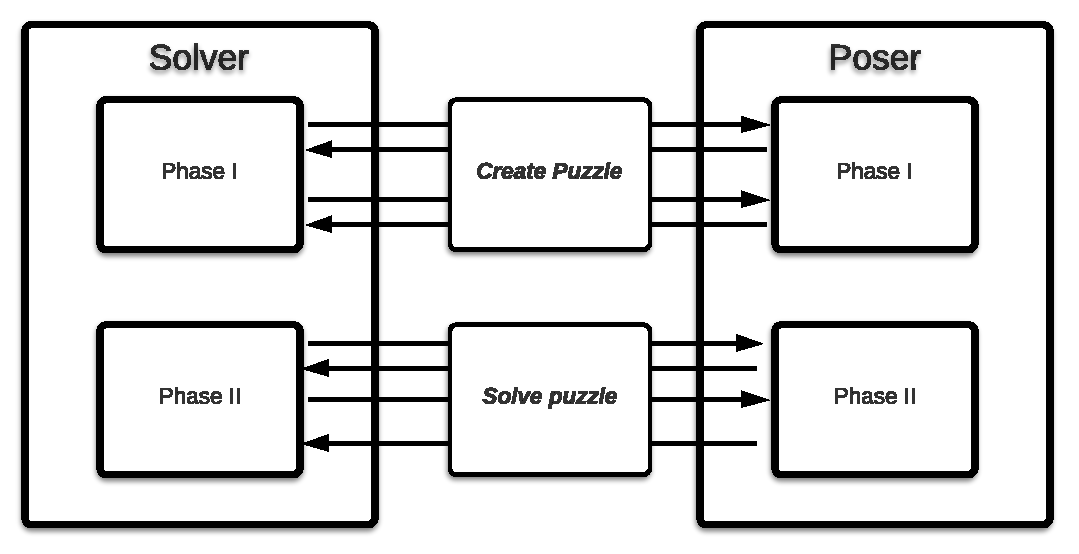
\includegraphics[scale=0.43]{images/IntProtocol.pdf}
  \end{figure}
\end{frame}

\begin{frame}[t]
  \frametitle{Hardness amplification results}
  \begin{itemize}
    \item<1-3> Weakly verifiable puzzles e.g. CAPTCHA, \cite{canetti2005hardness}
    \item<2-3> Dynamic weakly verifiable puzzles $+$ threshold functions e.g.~MAC,\cite{dodis2009security}
    \item<3> Interactive weakly verifiable puzzles $+$ monotone function e.g.~commitment protocols, \cite{holenstein2011general}
  \end{itemize}
  \centering
\end{frame}

\begin{frame}[t]
  \frametitle{Goal}
  \begin{itemize}
    \item Define puzzle that generalize MAC, CAPTCHA, bit commitments.
    \item Amplify hardness by parallel repetition.
  \end{itemize}
  \vspace{40pt}
  \begin{figure}
    \centering
    \begin{tikzpicture}[remember picture,overlay]
      % Weakly Verifiable box
      \node (rect) at (-4,0) [draw,thin, minimum width=3cm,minimum height=2.6cm, text width = 3cm, align=center] {
        Monotone functions
      };
      \node (plus) at (-2,0) {+};
      \node (rect) at (0,0) [draw,thin, minimum width=3cm,minimum height=2.6cm, text width = 3cm, align=center] {
        Dynamic weakly verifiable puzzles
      };
      \node (plus) at (2,0) {+};
      \node (rect3) at (4,0) [draw,thin, minimum width=3cm,minimum height=2.6cm, text width = 3cm, align=center] {
        Interactive weakly verifiable puzzles
      };
    \end{tikzpicture}
  \end{figure}
\end{frame}

\begin{frame}[t]
\frametitle{Reduction}
\begin{itemize}
  \item $A$ - solving a single puzzle is hard
  \item $B$ - solving parallel repetition is hard
    \begin{align*}
      A \implies B
    \end{align*}
      \begin{align*}
        \lnot B \implies \lnot A
      \end{align*}
  \item Given a good solver $C$ for parallel repetition
  \item Reduce $C$ to a solver for single puzzle
\end{itemize}
\end{frame}

% \begin{frame}[t]
% \frametitle{Problems}
% % TODO maybe block diagram?
% \begin{itemize}
%   \item Fix a position for the input puzzle
%   \item Generate $n-1$ puzzles
%   \item Run $C$ multiple times
%   \item If the solution is correct output it
%   \item One has to run $C$ multiple times
%   \item Hint query may prevent block a solution that would be correct
%   \item Not possible to check correctness of the solution for the input puzzle
% \end{itemize}
% \end{frame}

\begin{frame}[t]
  \frametitle{Problem: conflicting hint queries}
  \begin{itemize}
    \item<1-5> The solver $C$ can be run multiple times.
    \item<2-5> Hint queries prevent verification queries from succeeding.
    \item<3-5> Use hash function to partition query domain \cite{dodis2009security}.
    \item<4-5> Can ask hints only on $\cQ \setminus \cQ_{\mathit{verification}}$.
    \item<5> Substantial success probability for partitioned domain.
  \end{itemize}
  \onslide<3-5>
  \begin{columns}
    \begin{column}{.4\textwidth}
      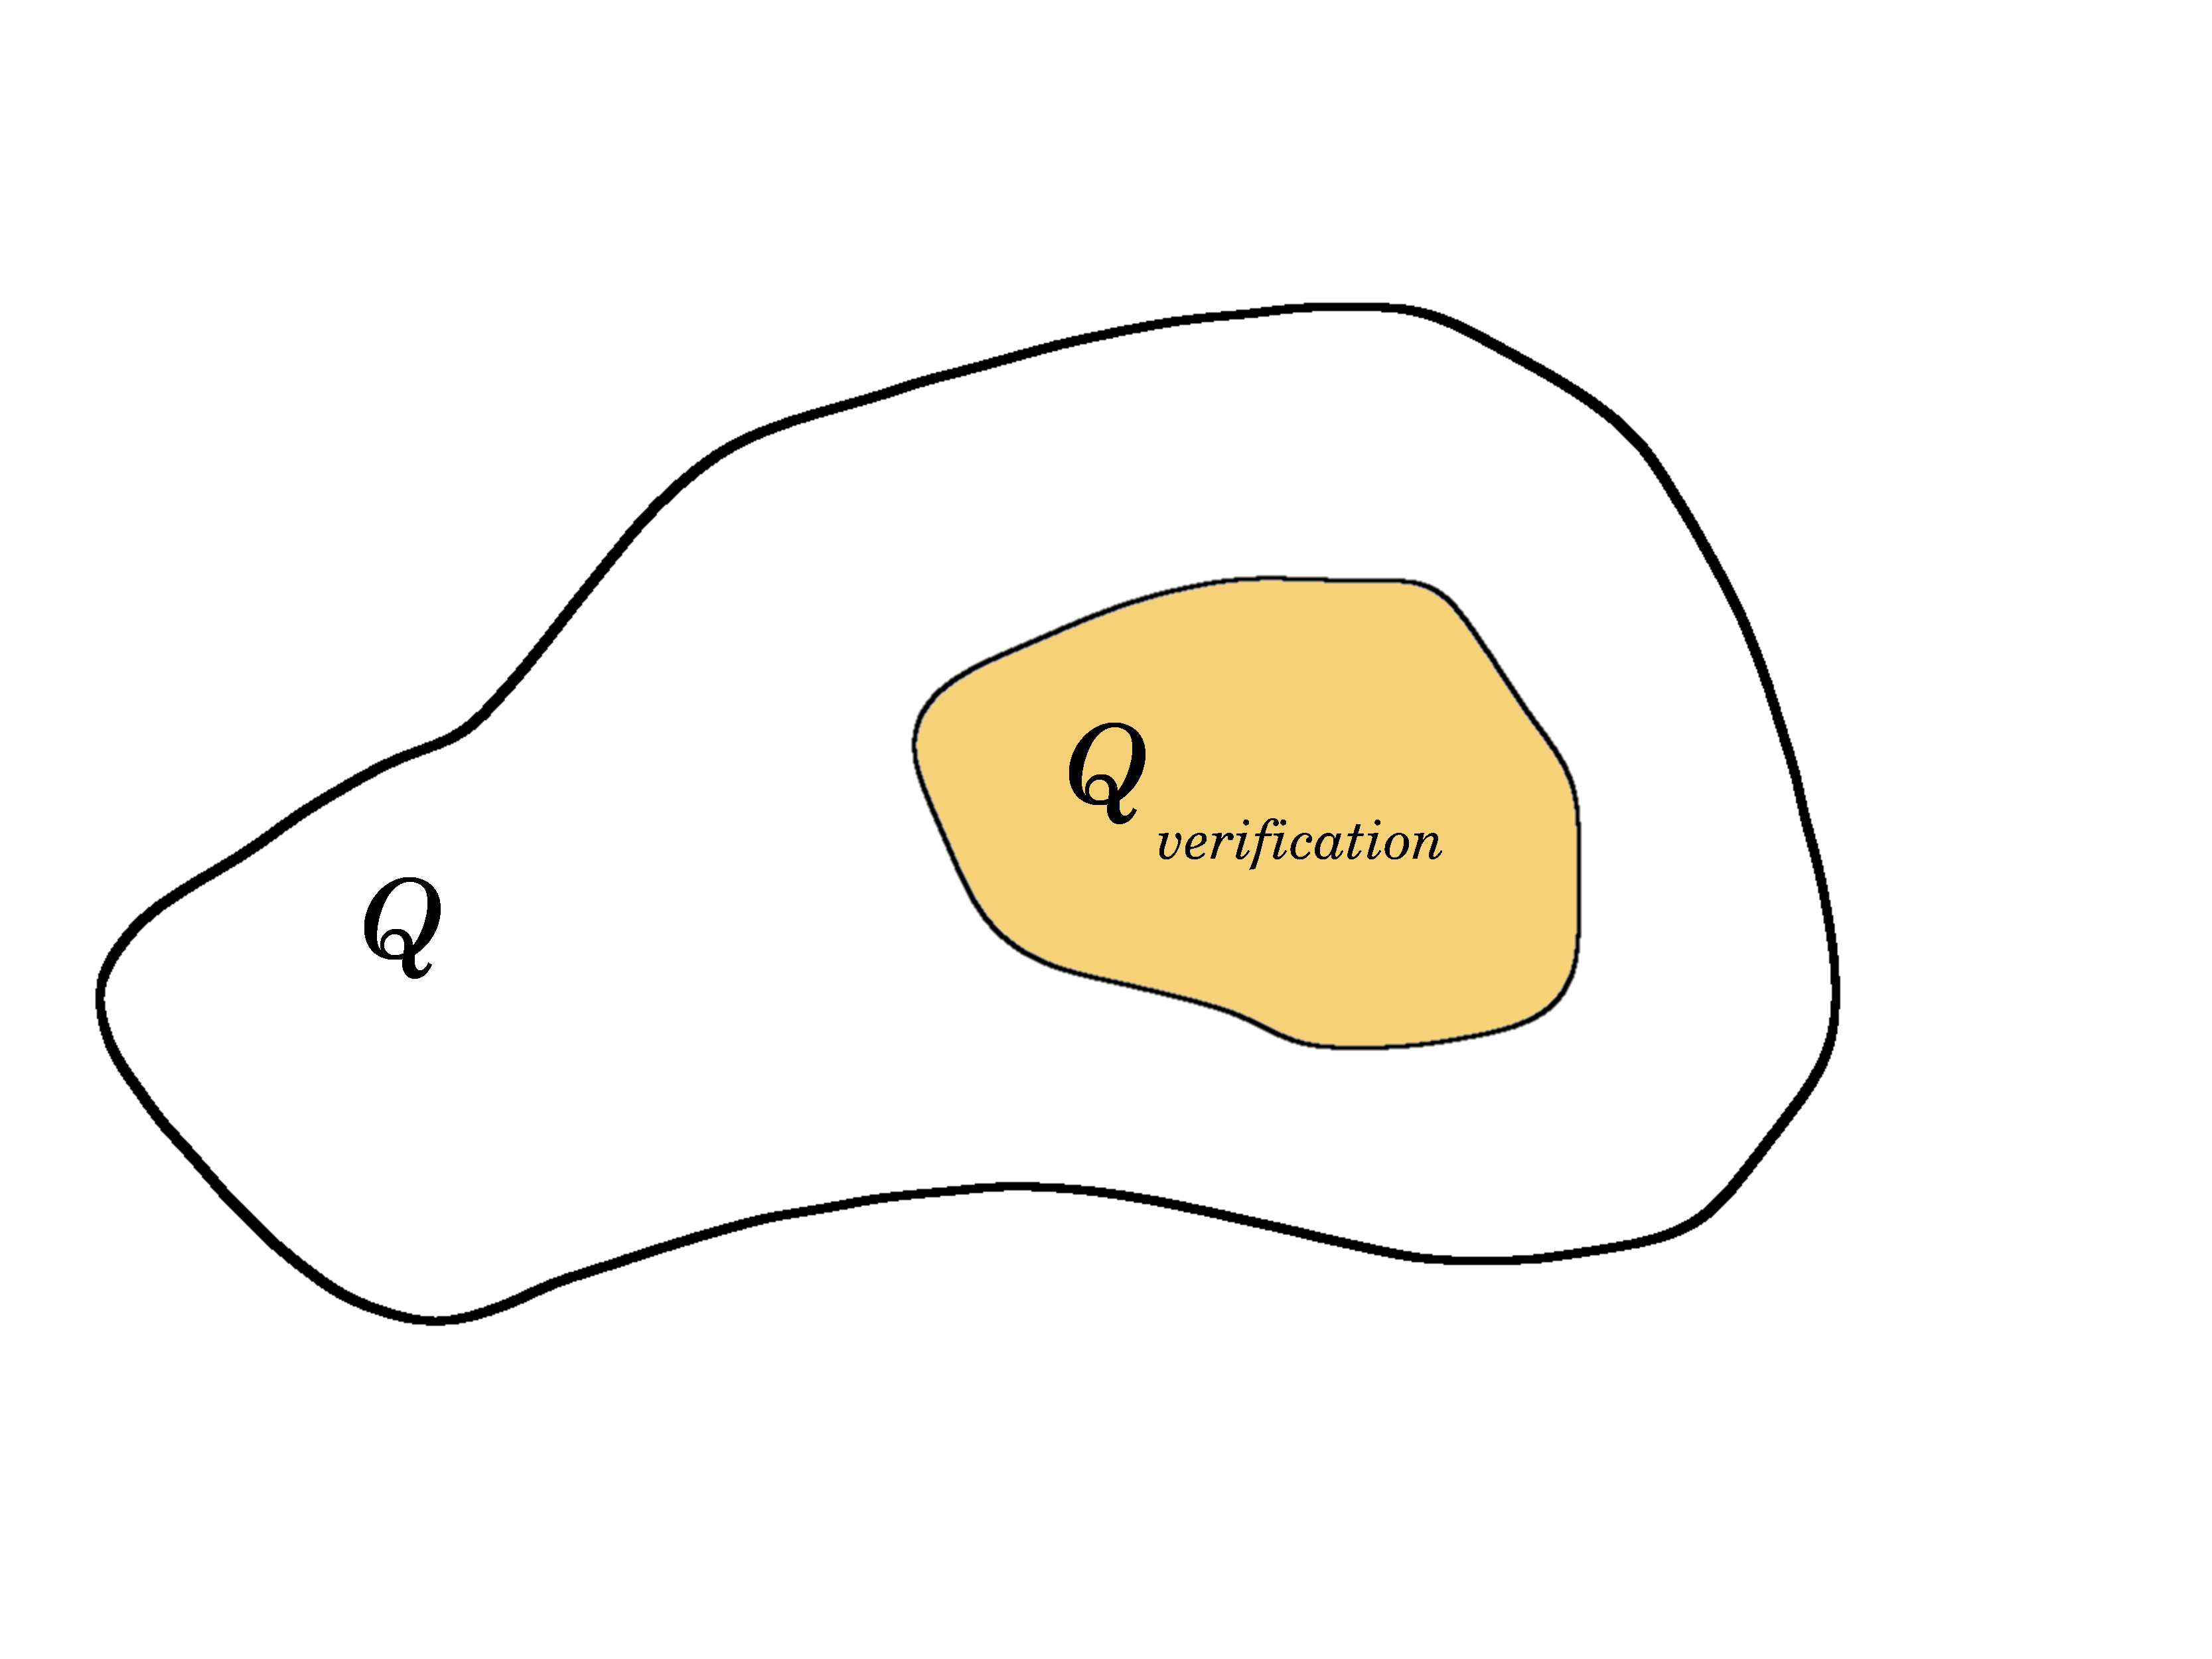
\includegraphics[scale=0.08]{images/hashSets.pdf}
    \end{column}
    \begin{column}{.4\textwidth}
      \begin{align*}
        &\hash \leftarrow \cH \\
        &\hash : \cQ \rightarrow \{0,1,\dots, 2(h+v) - 1\} \\
        &\cQ_{\mathit{verification}} := {q \in \cQ : hash(q) = 0}
      \end{align*}
    \end{column}
  \end{columns}
\end{frame}

\begin{frame}[t]
  \frametitle{Approach overview}
  \centering
  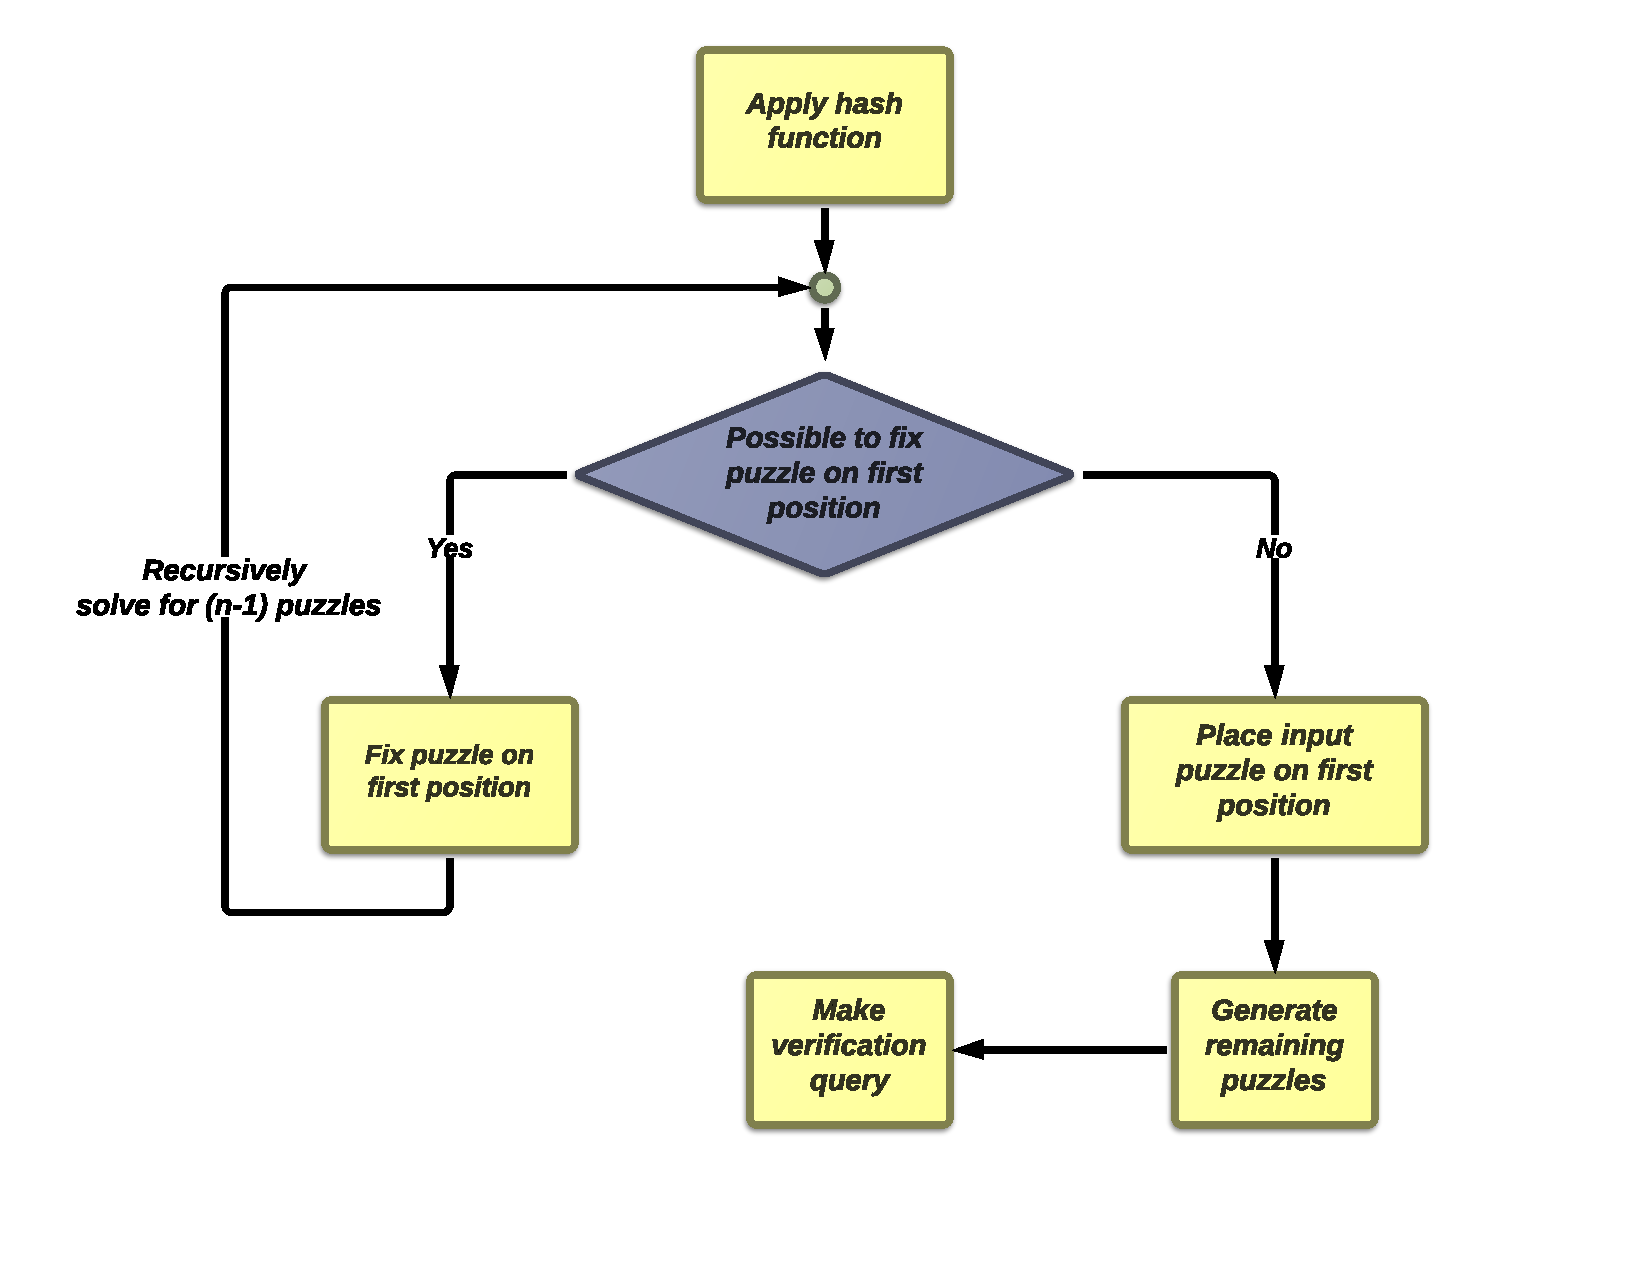
\includegraphics[scale=0.3]{images/AlgoBlock1.pdf}
\end{frame}

\begin{frame}[t]
  \frametitle{Problem: verifying the solution}
  \begin{columns}
    \begin{column}{.5\textwidth}
      \begin{itemize}
      \item<1-2> Cannot verify correctness of a solution for input puzzle.
      \item<2> Possible for generated puzzles.
      \end{itemize}
    \end{column}
    \begin{column}{.5\textwidth}
      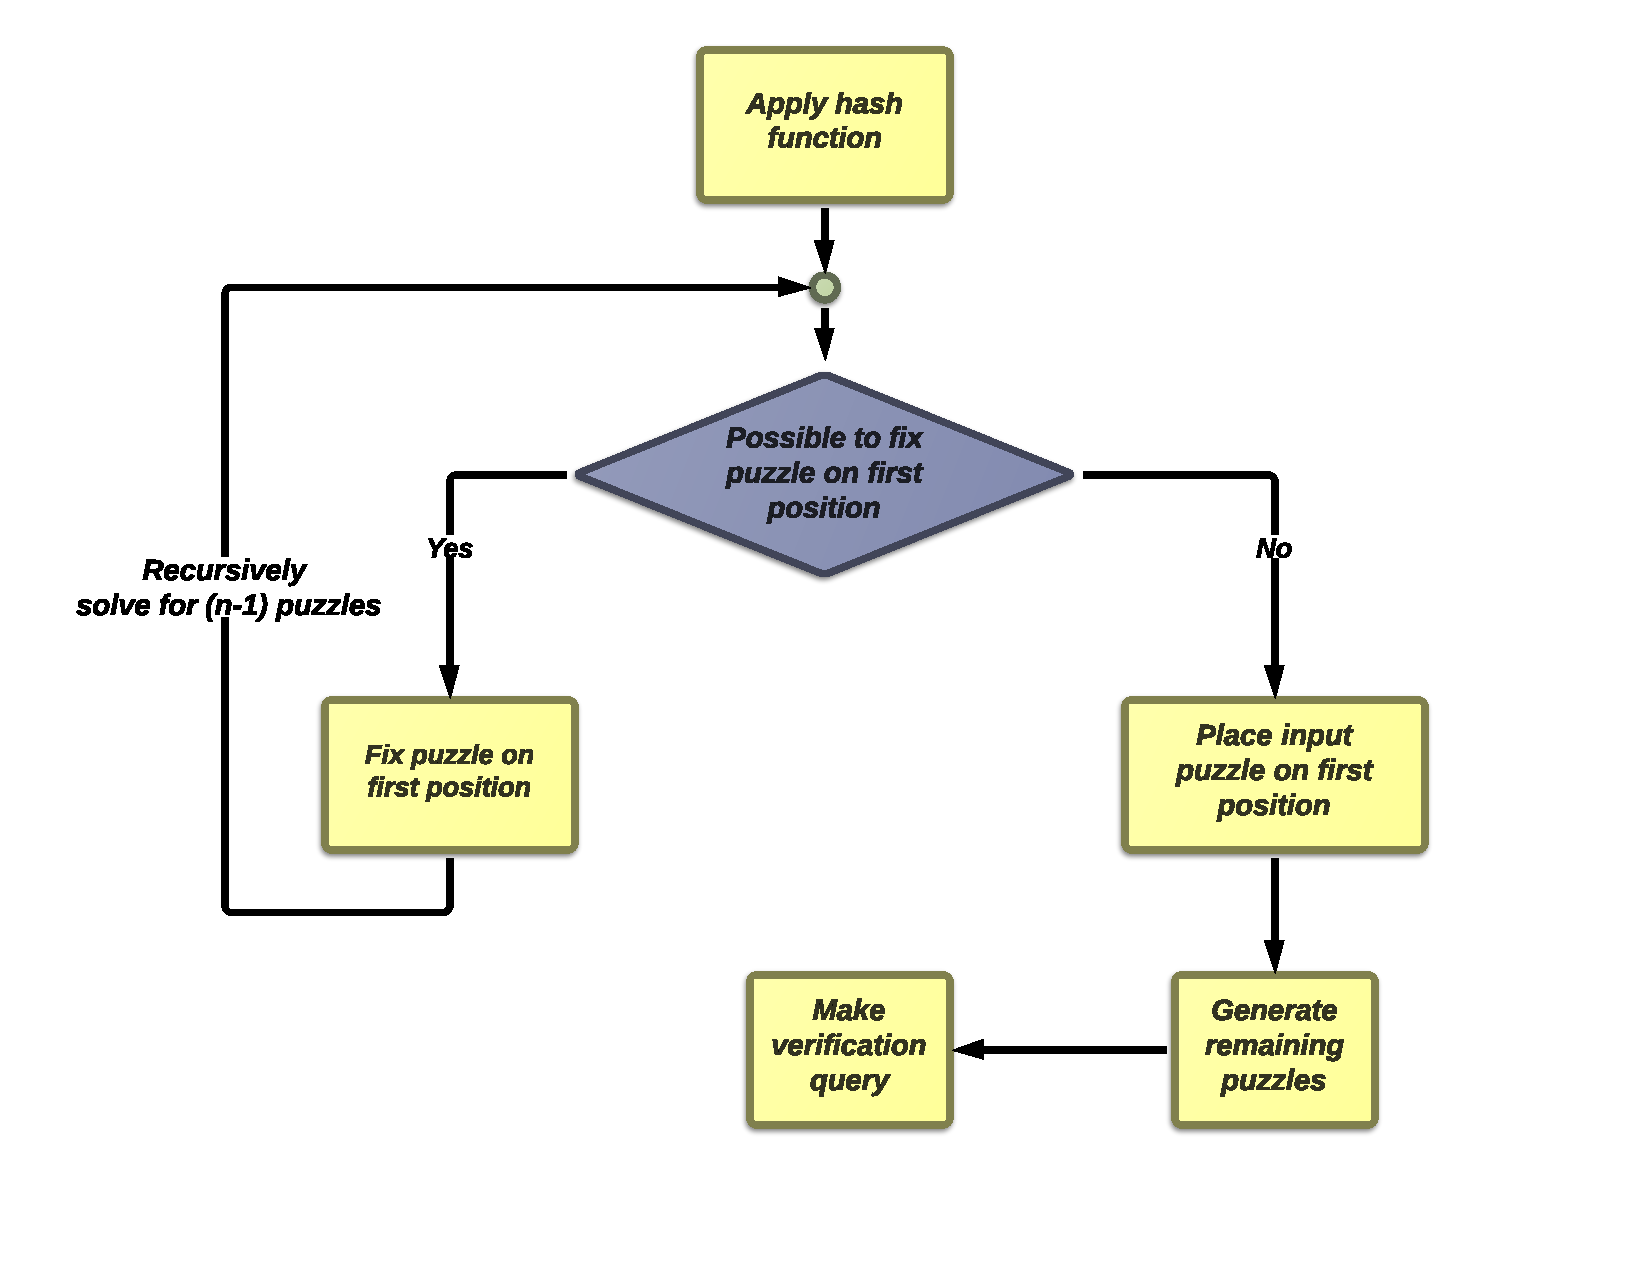
\includegraphics[scale=0.22]{images/AlgoBlock1.pdf}
    \end{column}
  \end{columns}
  \onslide<2>
  \[\begin{tikzpicture}[remember picture,overlay]
    \node (rect) at (-4,0) [draw,thin, minimum width=.6cm,minimum height=.6cm] {?};
    \node (rect) at (-3.4,0) [draw,thin, minimum width=.6cm,minimum height=.6cm] {1};
    \node (rect) at (-2.8,0) [draw,thin, minimum width=.6cm,minimum height=.6cm] {1};
    \draw[decorate sep={0.3mm}{3mm}, fill] (-2.2, 0) -- (-0.6, 0);
    \node (rect) at (0,0) [draw,thin, minimum width=.6cm,minimum height=.6cm] {1};
\draw [decorate,decoration={brace,amplitude=10pt,mirror,raise=4pt},yshift=0pt] (-4.3,-.2) -- (0.3,-.2) node at (-2,-1) {$\geq \delta^k$};
\draw [decorate,decoration={brace,amplitude=10pt,raise=4pt},yshift=0pt] (-3.4,0.3) -- (0.3,0.3) node at (-1.7,1) {$< \delta^{k-1}$};
  \end{tikzpicture}\]
\end{frame}

\begin{frame} [t]
  \frametitle{Result}
      Given a solver for parallel repetition of puzzles that satisfies\\
      \begin{align*}
        \geq \delta^k + \epsilon \text{\hspace{20pt\pause}(} \geq \Pr[g(u_1, \dots, u_k) = 1] + \varepsilon \text{)},
      \end{align*}
      where $\Pr[u_i = 1] = \delta$. \\
      \pause
      \vspace{25pt}
      We devise a solver for a single puzzle that satisfies (almost surely)
      \begin{align*}
         \geq \frac{1}{16(h+v)} \Bigl(\delta + \frac{\epsilon}{6k}\Bigr).
      \end{align*}
\end{frame}

\begin{frame}[t]
  \frametitle{Discussion}
  \begin{itemize}
    \item Not clear whether it is possible to improve the result
      \begin{align*}
         \geq \textcolor{orange}{\frac{1}{16(h+v)}} \Bigl(\delta + \frac{\epsilon}{6k}\Bigr).
      \end{align*}
      \pause
    \item Improve it? \pause \textcolor{orange}{\xmark}
    \item Is it optimal? \pause \textcolor{orange}{\xmark}
  \end{itemize}
\end{frame}

\begin{frame}
\frametitle{Questions}
\end{frame}


\begin{frame}[t]
\frametitle{Bibliography}
\bibliographystyle{alpha}
\bibliography{refs}
\end{frame}

\note{
  \begin{enumerate}
    \item What is weak one-way function:
      there exists a polynomial that lower bounds the failure probability of every polynomial time algorithm. Goldreich p.35.
    \item What is strong one-way function?

    \item Why it may not be optimal?

    \item What did you try to show that it is possible to improve your results?

    \item Is it computational or information theoretic result?

    \item What kind of security-games for MAC are modeled by DWVP?

    \item Why sequential repetition implies security amplification?

    \item What if the number of puzzles in the sequential repetition is very big i.e. our result holds only with high probability?

    \item Does repeating the whole algorithm may help and increase the success probability?

    \item What is the cryptographic primitive?

    \item What is the cryptographic scheme?

    \item Is there a simple proof for sequential repetition?

    \item Why is it not possible to fix all coordinates? Give examples in $n$-dim space.

    \item Try to justify why we have this form of the theorem, what does it mean? and what w
  \end{enumerate}
}

\note{
  \begin{enumerate}

  \item Where does the proof break when you want to apply it to the large surplus

  \item When does the proof breaks? -- exactly and why we do not have to care about it too much

  \item What it the intuition behind the surplus?

  \item Be manage to explain the function on the right hand-side.

  \item Why do we need to consider two surpluses

  \item How does the optimization problem for gap amplification looks like?

  \item Why we cannot perfect hardness amplification?

  \item Why $\Pr[c \in \cG_1 \setminus \cG_0]$ is small but we still have a large surplus

  \item Why can we assume that the verification algorithm can be deterministic

  \item Followup question: what is proven in DIJK09

  \item Followup question: why is the hint circuit H probabilistic

  \item Is defining the puzzle only by poser is not artificial as an instance is defined by a pair poser-solver

  \item There are no examples of puzzles that are both interactive and dynamic what about this?

  \item Number of rounds for which parallel repetition works as i.e. the intuition behind the > 3-round protocols

  \end{enumerate}
}


\note {
  \begin{enumerate}

  \item Why does obsevation 5.1 is true?

  \item What is function what is relation

  \item Why WVP does not imply one-way function

  \item Is it possible that sampling does not work?

  \item Is number of hint and verification queries limitation for the solver or the verify

  \item Why do we iterate $\frac{1}{\epsilon}$ times in $\Gen$, is it efficient, when it might not be efficient what happens with $h+v$ then?

  \item Think about different computational contexts for this theorem. Under what conditions for $h,v,\epsilon$ does it make sense

  \item Be able to explain the definition in DIJK09.

  \item What is the Coron's proof about? Why it does not work?

  \item $k$-wise independent functions; how do they look like?

  \item Random questions about hash functions

  \item (if not covered in the presentation) is your result optimal?

  \item Relation with soundness error of four-round protocols

  \end{enumerate}
}
\end{document}